\documentclass[12pt]{article}

\usepackage[a4paper,margin=1in]{geometry}
\usepackage[utf8]{inputenc}
\usepackage[spanish,es-tabla]{babel}
\usepackage{graphicx}
\usepackage[american]{circuitikz}
\usepackage{amsmath}
\usepackage{subcaption}
\usepackage{amssymb}
\usepackage[hidelinks]{hyperref}
\usepackage{mathtools}
\usepackage{enumitem}
\usepackage{array}
\usepackage{longtable}
\usepackage{multirow}
\usepackage{csquotes}
\usepackage{float}
\usepackage{setspace}
\usepackage{pgfplots}
\pgfplotsset{compat=1.18}
\usetikzlibrary{arrows.meta, decorations.pathreplacing, calc, positioning}
\usepackage[style=ieee, backend=bibtex]{biblatex}
\addbibresource{bibliografia.bib}
\graphicspath{{Figuras/}{../figs/}}
\onehalfspacing

\hypersetup{
    colorlinks=true,
    linkcolor=blue,
    citecolor=blue,
    urlcolor=blue,
    filecolor=blue
}

\begin{document}
\renewcommand{\figureautorefname}{Fig.}
\renewcommand{\tableautorefname}{Tab.}
\renewcommand{\equationautorefname}{Ec.}

\begin{titlepage}
\thispagestyle{empty}
\begin{tikzpicture}[remember picture,overlay]
    \node[opacity=0.2,anchor=center] at (current page.center)
        {
\includegraphics[width=0.9\paperwidth]{decoracion_a.png}};
\end{tikzpicture}
\begin{center}
    
\includegraphics[width=15cm]{unc_fcefyn_logo.png} \\ [0.5cm]
    \LARGE Universidad Nacional de Córdoba \\ [0.5cm]
    \large Facultad de Ciencias Exactas, Físicas y Naturales \\
    \vspace{40pt}
    \large Síntesis de Redes Activas \\ [0.2cm]
    \large Trabajo Práctico de Laboratorio N°4 \\
    \vspace{60pt}
    \LARGE Filtros Activos\\
    \vspace{60pt}
    \begin{table}[!h]
        \centering
        \begin{tabular}{ll}
            \multicolumn{1}{c}{Nombre} & \multicolumn{1}{c}{DNI} \\
            Arteaga Barrera, Cristian Eduardo & 95.159.096 \\
            Baccino, Luca                     & 45.328.380 \\
            Baccino, Octavio                  & 44.350.820
        \end{tabular}
    \end{table}
    \vspace{20pt}
    \begin{table}[!h]
        \centering
        \begin{tabular}{ll}
            \multicolumn{1}{c}{Docentes} & Dr. Ing. Ferreyra, Pablo \\
                                         & Ing. Reale, César \\
        \end{tabular}
    \end{table}
    \vfill
        {\small Córdoba, República Argentina\\
                Año 2026}
\end{center}
\end{titlepage}
\newpage

\tableofcontents
\newpage
\listoffigures
\newpage
\listoftables
\newpage

\section{Introducción}
\label{sec_1}
El presente trabajo práctico aborda la síntesis de un filtro activo pasabanda a partir de una plantilla de requerimientos de atenuación provista por la Cátedra \cite{guia}. El filtro debe dejar pasar la banda comprendida entre $800 \, [Hz]$ y $1250 \, [Hz]$ con una atenuación máxima de $0.25 \, [dB]$, y atenuar al menos $30 \, [dB]$ las frecuencias inferiores a $200 \, [Hz]$ y superiores a $5 \, [kHz]$.

El diseño se realiza aproximando la función de atenuación mediante polinomios de Chebyshev y sintetizando la función de transferencia resultante con dos secciones bicuadráticas \textit{Sallen-Key} de realimentación positiva implementadas con amplificadores operacionales LM324. Sobre el circuito obtenido se calculan las sensibilidades de la frecuencia del polo y del ancho de banda de cada bicuadrática, se analiza la peor desviación con componentes de $10 \, [\%]$ de tolerancia y se realiza una simulación de Montecarlo en LTspice \cite{ltspice}.

El trabajo se organiza de la siguiente manera. En la \autoref{sec_2} se presentan los fundamentos teóricos. En la \autoref{sec_3} se desarrollan la aproximación, la síntesis del circuito, las simulaciones y los análisis de sensibilidad y tolerancia, junto con las condiciones de operación límite. En la \autoref{sec_4} se resuelve el ejercicio adicional: un oscilador senoidal de $12 \, [kHz]$. Finalmente, en la \autoref{sec_5} se presentan las conclusiones.

\section{Marco Teórico}
\label{sec_2}

\subsection{Aproximación de Chebyshev}
\label{sec_2.1}
El problema de la aproximación consiste en encontrar una función de transferencia realizable cuya respuesta en módulo quede contenida dentro de la plantilla de requerimientos. La aproximación de Chebyshev (tipo I) propone, para el filtro pasabajos normalizado, una respuesta de la forma \cite{huelsman, schaumann}:
\begin{equation}
    |H(j\Omega)|^2 = \frac{1}{1 + \varepsilon^2 \, C_n^2(\Omega)}
    \label{eq:cheby}
\end{equation}
donde $C_n(\Omega)$ es el polinomio de Chebyshev de orden $n$, que oscila entre $-1$ y $1$ para $|\Omega| \leq 1$ y crece monótonamente para $|\Omega| > 1$:
\begin{equation}
    C_n(\Omega) =
    \begin{cases}
        \cos\left(n \arccos \Omega\right)            & |\Omega| \leq 1 \\
        \cosh\left(n \, \mathrm{arccosh} \, \Omega\right) & |\Omega| > 1
    \end{cases}
\end{equation}

En consecuencia, la atenuación en la banda de paso oscila entre $0$ y $A_p$ (\textit{equiripple}), donde el parámetro $\varepsilon$ fija la amplitud del rizado:
\begin{equation}
    \varepsilon = \sqrt{10^{A_p/10} - 1}
    \label{eq:eps}
\end{equation}

Exigiendo una atenuación mínima $A_s$ en la frecuencia normalizada de rechazo $\Omega_s$, el orden mínimo necesario resulta:
\begin{equation}
    n \geq \frac{\mathrm{arccosh}\sqrt{\dfrac{10^{A_s/10} - 1}{10^{A_p/10} - 1}}}{\mathrm{arccosh} \, \Omega_s}
    \label{eq:orden}
\end{equation}

Frente a la aproximación de Butterworth, la de Chebyshev concentra el error de aproximación de manera uniforme en toda la banda de paso, lo que le permite lograr una transición más abrupta con el mismo orden. Como contrapartida, sus polos poseen factores de calidad más elevados.

\subsection{Transformación Pasabajos -- Pasabanda}
\label{sec_2.2}
El filtro pasabanda se obtiene a partir del prototipo pasabajos normalizado mediante la transformación de frecuencia \cite{huelsman}:
\begin{equation}
    s_{PB} = \frac{s^2 + \omega_0^2}{B \, s}, \qquad \omega_0 = \sqrt{\omega_{p1} \, \omega_{p2}}, \qquad B = \omega_{p2} - \omega_{p1}
    \label{eq:transf}
\end{equation}
donde $\omega_{p1}$ y $\omega_{p2}$ son los bordes de la banda de paso. La transformación duplica el orden: cada par de polos complejos del prototipo genera dos pares de polos del pasabanda, ubicados de forma geométricamente simétrica respecto de $\omega_0$. La frecuencia de rechazo normalizada del prototipo se obtiene como:
\begin{equation}
    \Omega_s = \min_{i} \frac{\left|\omega_{s,i}^2 - \omega_0^2\right|}{B \, \omega_{s,i}}
    \label{eq:omegas}
\end{equation}

\subsection{Secciones Bicuadráticas Sallen-Key}
\label{sec_2.3}
Una función de transferencia de orden par puede factorizarse en el producto de funciones de segundo orden (bicuadráticas), cada una caracterizada por la frecuencia del polo $\omega_p$ y su factor de calidad $Q_p$:
\begin{equation}
    T(s) = \prod_{i} \frac{N_i(s)}{s^2 + \dfrac{\omega_{p,i}}{Q_{p,i}} \, s + \omega_{p,i}^2}
\end{equation}

Cada sección se implementa con una celda activa y luego se conectan en cascada. Dado que la impedancia de salida de un amplificador operacional realimentado es prácticamente nula, las etapas no se cargan entre sí y la transferencia total es el producto de las individuales.

La topología \textit{Sallen-Key} \cite{sallenkey} utiliza realimentación positiva a través de un capacitor (pasabajos) o una resistencia (pasaaltos) conectado a la salida de un amplificador de ganancia $K$. En este trabajo se emplea la variante de \textbf{ganancia unitaria} ($K = 1$, seguidor de tensión), que es la menos sensible a las variaciones de los componentes y no requiere resistencias adicionales en la red de realimentación negativa.

\begin{figure}[H]
    \centering
    \begin{subfigure}{0.49\textwidth}
        \centering
        \begin{circuitikz}[scale=0.75, transform shape]
            \draw (5.2,0) node[op amp, noinv input up, anchor=+] (U) {};
            \draw (0,0) node[left]{$V_i$} to[R, l=$R_1$, o-*] (2,0) to[R, l=$R_2$, -*] (4,0) -- (U.+);
            \draw (4,0) to[C, l_=$C_2$] (4,-2) node[ground]{};
            \draw (2,0) -- (2,2) to[C, l=$C_1$] ($(U.out)+(0.5,2)$) |- (U.out);
            \draw (U.-) -- ++(-0.3,0) |- ($(U.out)+(0,-1.3)$) -- (U.out);
            \draw (U.out) to[short, *-o] ++(1,0) node[right]{$V_o$};
        \end{circuitikz}
        \caption{Pasabajos.}
        \label{fig:sk_pb}
    \end{subfigure}
    \hfill
    \begin{subfigure}{0.49\textwidth}
        \centering
        \begin{circuitikz}[scale=0.75, transform shape]
            \draw (5.2,0) node[op amp, noinv input up, anchor=+] (U) {};
            \draw (0,0) node[left]{$V_i$} to[C, l=$C_3$, o-*] (2,0) to[C, l=$C_4$, -*] (4,0) -- (U.+);
            \draw (4,0) to[R, l_=$R_4$] (4,-2) node[ground]{};
            \draw (2,0) -- (2,2) to[R, l=$R_3$] ($(U.out)+(0.5,2)$) |- (U.out);
            \draw (U.-) -- ++(-0.3,0) |- ($(U.out)+(0,-1.3)$) -- (U.out);
            \draw (U.out) to[short, *-o] ++(1,0) node[right]{$V_o$};
        \end{circuitikz}
        \caption{Pasaaltos.}
        \label{fig:sk_pa}
    \end{subfigure}
    \caption{Celdas bicuadráticas Sallen-Key de ganancia unitaria.}
    \label{fig:sk}
\end{figure}

Para el \textbf{pasabajos} de la \autoref{fig:sk_pb}, con $R_1$ y $R_2$ en serie y $C_1$ conectado a la salida, el análisis nodal conduce a:
\begin{equation}
    T_{PB}(s) = \frac{\dfrac{1}{R_1 R_2 C_1 C_2}}{s^2 + \dfrac{R_1 + R_2}{R_1 R_2 C_1} \, s + \dfrac{1}{R_1 R_2 C_1 C_2}}, \qquad
    \omega_p = \frac{1}{\sqrt{R_1 R_2 C_1 C_2}}, \qquad
    Q_p = \frac{\sqrt{R_1 R_2 C_1 C_2}}{C_2 \left(R_1 + R_2\right)}
    \label{eq:sk_pb}
\end{equation}

Para el \textbf{pasaaltos} de la \autoref{fig:sk_pa}, con $C_3$ y $C_4$ en serie, $R_3$ conectada a la salida y $R_4$ a masa:
\begin{equation}
    T_{PA}(s) = \frac{s^2}{s^2 + \dfrac{C_3 + C_4}{R_4 C_3 C_4} \, s + \dfrac{1}{R_3 R_4 C_3 C_4}}, \qquad
    \omega_p = \frac{1}{\sqrt{R_3 R_4 C_3 C_4}}, \qquad
    Q_p = \frac{\sqrt{R_3 R_4 C_3 C_4}}{R_3 \left(C_3 + C_4\right)}
    \label{eq:sk_pa}
\end{equation}

Con $R_1 = R_2$ en el pasabajos y $C_3 = C_4$ en el pasaaltos, el factor de calidad depende sólo de un cociente de componentes:
\begin{equation}
    Q_{PB} = \frac{1}{2}\sqrt{\frac{C_1}{C_2}}, \qquad Q_{PA} = \frac{1}{2}\sqrt{\frac{R_4}{R_3}}
    \label{eq:q_cociente}
\end{equation}
por lo que un $Q_p$ elevado exige una dispersión de valores de $4 Q_p^2$.

\subsection{Sensibilidad y Tolerancias}
\label{sec_2.4}
La sensibilidad relativa de un parámetro $y$ respecto de un elemento $x$ se define como \cite{schaumann}:
\begin{equation}
    S_x^y = \frac{x}{y} \, \frac{\partial y}{\partial x} \approx \frac{\Delta y / y}{\Delta x / x}
    \label{eq:sens}
\end{equation}
y cumple las propiedades $S_x^{y_1 y_2} = S_x^{y_1} + S_x^{y_2}$, $S_x^{1/y} = -S_x^y$ y $S_x^{y^k} = k \, S_x^y$. Para una variación de todos los componentes, la desviación relativa de $y$ se aproxima a primer orden por:
\begin{equation}
    \frac{\Delta y}{y} \approx \sum_i S_{x_i}^{y} \, \frac{\Delta x_i}{x_i}
    \qquad \Rightarrow \qquad
    \left|\frac{\Delta y}{y}\right|_{max} \approx \delta \sum_i \left|S_{x_i}^{y}\right|
    \label{eq:peor}
\end{equation}
donde $\delta$ es la tolerancia de los componentes. El peor caso se da cuando cada componente se desvía hacia el extremo de su tolerancia que hace que su contribución tenga el mismo signo que las demás.

El análisis de peor caso es conservador, ya que la probabilidad de que todos los componentes se ubiquen simultáneamente en el extremo desfavorable es muy baja. La simulación de \textbf{Montecarlo} complementa este análisis asignando a cada componente un valor aleatorio dentro de su tolerancia y repitiendo la simulación un número elevado de veces, lo que permite estimar la dispersión estadística de la respuesta y el rendimiento de fabricación (porcentaje de circuitos que cumplen la especificación).

\newpage

\section{Desarrollo}
\label{sec_3}

\subsection{Plantilla de Requerimientos}
\label{sec_3.0}
La plantilla de la Cátedra \cite{guia} establece los siguientes requerimientos:
\begin{itemize}
    \item \underline{Banda de paso:} $f_{p1} = 800 \, [Hz]$ a $f_{p2} = 1250 \, [Hz]$, con atenuación máxima $A_p = 0.25 \, [dB]$.
    \item \underline{Bandas de rechazo:} $f < f_{s1} = 200 \, [Hz]$ y $f > f_{s2} = 5000 \, [Hz]$, con atenuación mínima $A_s = 30 \, [dB]$.
\end{itemize}

Se observa que $f_{s1} \, f_{s2} = f_{p1} \, f_{p2} = 10^6 \, [Hz^2]$, es decir, la plantilla es geométricamente simétrica respecto de la frecuencia central $f_0 = \sqrt{f_{p1} f_{p2}} = 1000 \, [Hz]$. Todos los cálculos numéricos se realizaron en Python con la biblioteca \textit{SciPy}, cuyas funciones \texttt{cheb1ord} y \texttt{cheby1} son equivalentes a las de Matlab propuestas en el anexo de la guía; los scripts se encuentran en la carpeta \texttt{TP4/scripts} del repositorio.

\subsection{Aproximación de Chebyshev}
\label{sec_3.1}
A partir de la \autoref{eq:eps}, el parámetro de rizado es:
\begin{equation}
    \varepsilon = \sqrt{10^{0.25/10} - 1} = 0.2434
\end{equation}

El ancho de banda es $B = 2\pi \, (1250 - 800) = 2827.43 \, [rad/s]$ y la frecuencia central $\omega_0 = 2\pi \cdot 1000 = 6283.19 \, [rad/s]$. Por la simetría geométrica de la plantilla, ambos bordes de rechazo conducen a la misma frecuencia normalizada (\autoref{eq:omegas}):
\begin{equation}
    \Omega_s = \frac{5000^2 - 1000^2}{5000 \cdot 450} = \frac{1000^2 - 200^2}{200 \cdot 450} = 10.67
\end{equation}

Reemplazando en la \autoref{eq:orden}:
\begin{equation}
    n \geq \frac{\mathrm{arccosh}\sqrt{\dfrac{10^{3} - 1}{10^{0.025} - 1}}}{\mathrm{arccosh} \, 10.67} = \frac{5.560}{3.059} = 1.82 \quad \Rightarrow \quad n = 2
\end{equation}

El prototipo pasabajos normalizado de Chebyshev de orden $2$ con $A_p = 0.25 \, [dB]$ resulta:
\begin{equation}
    H_{LP}(s) = \frac{2.0541}{s^2 + 1.7967 \, s + 2.1140}
\end{equation}
cuya ganancia en continua es $2.0541/2.1140 = 0.9717$ ($-0.25 \, [dB]$), como corresponde a un filtro de Chebyshev de orden par. Aplicando la transformación de la \autoref{eq:transf} se obtiene el pasabanda de orden $4$:
\begin{equation}
    T(s) = \frac{1.64209 \times 10^{7} \, s^2}{s^4 + 5080.00 \, s^3 + 9.58572 \times 10^{7} \, s^2 + 2.00550 \times 10^{11} \, s + 1.55855 \times 10^{15}}
    \label{eq:T}
\end{equation}

Los polos de la \autoref{eq:T} y sus parámetros se presentan en la \autoref{tab:polos}. Factorizando, la función de transferencia coincide con la indicada en la plantilla de la Cátedra:
\begin{equation}
    T(s) = \frac{5252.26 \, s}{s^2 + 3184.42 \, s + 66320656} \cdot \frac{3126.49 \, s}{s^2 + 1895.58 \, s + 23500096}
\end{equation}

\begin{table}[H]
    \centering
    \caption{Polos de la función de transferencia aproximada.}
    \label{tab:polos}
    \begin{tabular}{|c|c|c|c|c|}
        \hline
        \textbf{Par de polos} & \textbf{Ubicación $[rad/s]$} & $\boldsymbol{f_p \, [Hz]}$ & $\boldsymbol{Q_p}$ & $\boldsymbol{\omega_p / Q_p \, [rad/s]}$ \\
        \hline
        Bajo & $-947.79 \pm j \, 4754.13$  & $771.53$  & $2.557$ & $1895.58$ \\
        Alto & $-1592.21 \pm j \, 7986.59$ & $1296.12$ & $2.557$ & $3184.43$ \\
        \hline
    \end{tabular}
\end{table}

Ambos pares tienen el mismo factor de calidad, consecuencia de la simetría geométrica de la transformación pasabanda. La atenuación en $200 \, [Hz]$ y en $5 \, [kHz]$ es de $34.83 \, [dB]$, de modo que el orden $2$ satisface la plantilla con un margen de $4.83 \, [dB]$ en la banda de rechazo. La respuesta se muestra en la \autoref{fig:aprox}.

\begin{figure}[H]
    \centering
    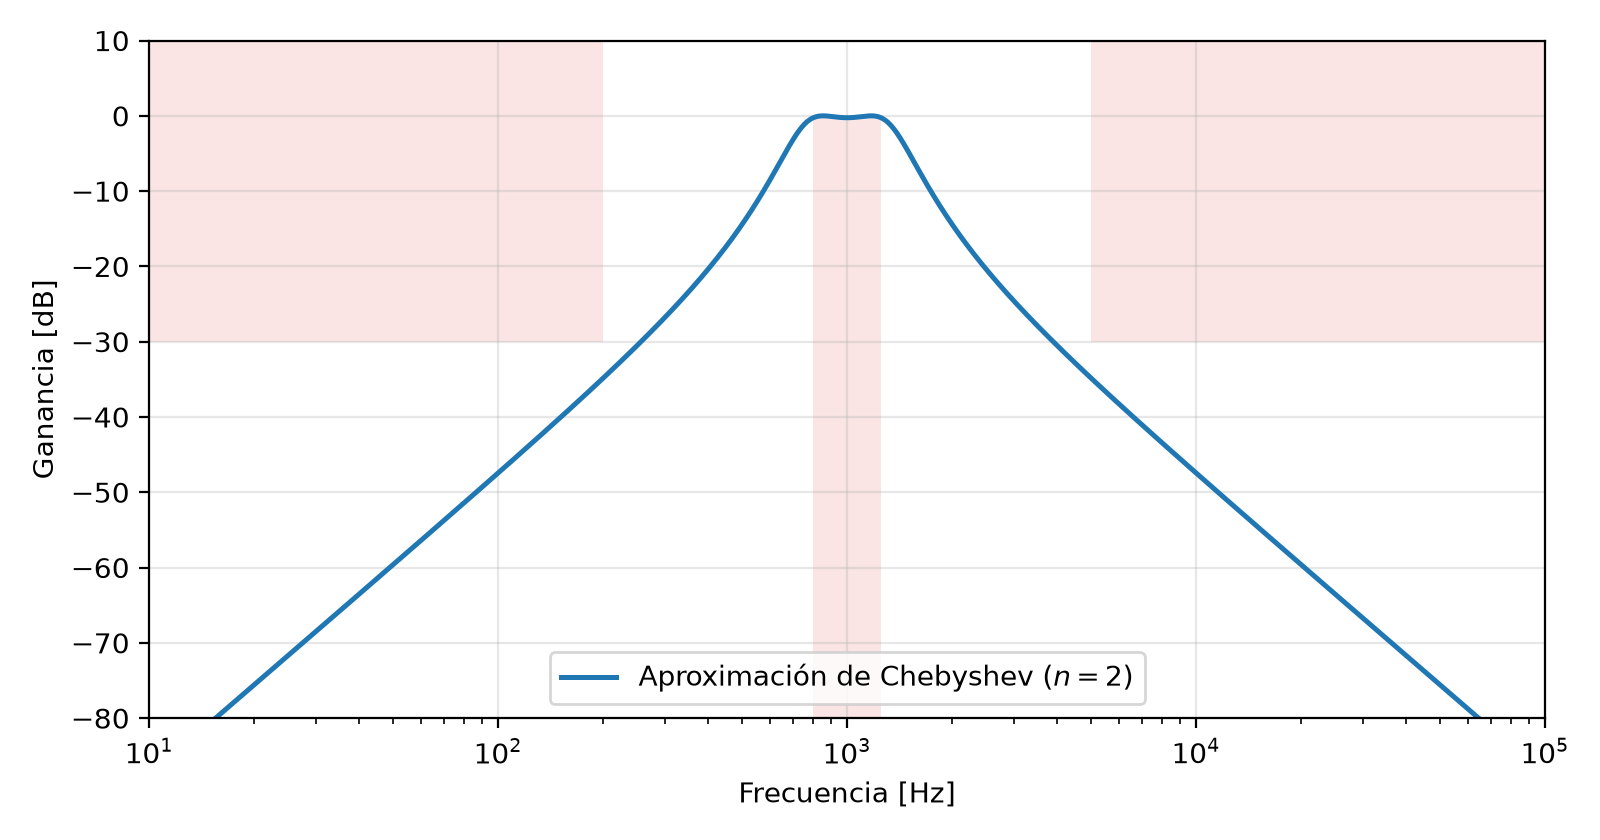
\includegraphics[width=0.85\textwidth]{aproximacion_chebyshev.png}
    \caption{Respuesta en frecuencia de la aproximación de Chebyshev y de cada etapa, junto con la plantilla de requerimientos (zonas sombreadas).}
    \label{fig:aprox}
\end{figure}

\subsection{Síntesis del Circuito}
\label{sec_3.2}

\subsubsection{Descomposición en Bicuadráticas}
Siguiendo la propuesta del anexo de la guía, la función de transferencia se implementa como la cascada de un pasabajos y un pasaaltos de segundo orden. El numerador $K s^2$ admite dos asignaciones de los pares de polos; se elige asignar el par bajo al pasabajos y el par alto al pasaaltos:
\begin{equation}
    T(s) = \underbrace{\frac{\alpha \, \omega_L^2}{s^2 + \dfrac{\omega_L}{Q} s + \omega_L^2}}_{\text{Pasabajos}} \cdot \underbrace{\frac{s^2}{s^2 + \dfrac{\omega_H}{Q} s + \omega_H^2}}_{\text{Pasaaltos}},
    \qquad \alpha = \frac{K}{\omega_L^2} = \frac{1.64209 \times 10^7}{23500096} = 0.6988
    \label{eq:alfa}
\end{equation}

Con esta asignación, dos etapas de ganancia unitaria producirían una ganancia de $1/\alpha = +3.11 \, [dB]$ en la banda de paso, por lo que basta una atenuación de entrada de $\alpha = -3.11 \, [dB]$ para normalizarla. La asignación opuesta exigiría $\alpha = K / \omega_H^2 = 0.2476$ ($-12.1 \, [dB]$), con mayores ganancias internas y menor rango dinámico.

La atenuación $\alpha$ se obtiene reemplazando $R_1$ del pasabajos por un divisor resistivo $R_a$--$R_b$ cuyo equivalente de Thévenin es:
\begin{equation}
    R_1 = R_a \parallel R_b, \qquad \alpha = \frac{R_b}{R_a + R_b} \qquad \Rightarrow \qquad R_a = \frac{R_1}{\alpha}, \qquad R_b = \frac{R_1}{1 - \alpha}
\end{equation}
de forma que no se agregan componentes activos ni se modifican $\omega_p$ y $Q_p$.

\subsubsection{Etapa Pasabajos}
De la \autoref{eq:q_cociente}, para $Q = 2.557$ se requiere $C_1 / C_2 = 4 Q^2 = 26.16$. Se eligen capacitores de la serie E12 $C_1 = 47 \, [nF]$ y $C_2 = 1.8 \, [nF]$ (cociente $26.11$), y con ellos:
\begin{equation}
    R = \frac{1}{\omega_L \sqrt{C_1 C_2}} = \frac{1}{4847.69 \cdot \sqrt{47 \, [nF] \cdot 1.8 \, [nF]}} = 22.43 \, [k\Omega]
\end{equation}

Para minimizar el error al normalizar las resistencias a la serie E96 ($1 \, [\%]$), se realizó una búsqueda sobre los valores normalizados vecinos admitiendo $R_1 \neq R_2$, lo que permite corregir levemente $Q_p$ mediante el cociente $R_1/R_2$ (\autoref{eq:sk_pb}). Se obtuvo $R_2 = 23.2 \, [k\Omega]$, $R_a = 30.9 \, [k\Omega]$ y $R_b = 73.2 \, [k\Omega]$ ($R_1 = 21.73 \, [k\Omega]$, $\alpha = 0.703$).

\subsubsection{Etapa Pasaaltos}
De la \autoref{eq:q_cociente}, $R_4 / R_3 = 4 Q^2 = 26.16$. Con $C_3 = C_4 = 12 \, [nF]$:
\begin{equation}
    \sqrt{R_3 R_4} = \frac{1}{\omega_H \, C} = 10.23 \, [k\Omega] \qquad \Rightarrow \qquad R_3 = 2.00 \, [k\Omega], \quad R_4 = 52.3 \, [k\Omega]
\end{equation}

\subsubsection{Circuito Final}
El circuito completo se muestra en la \autoref{fig:circuito}, y la \autoref{tab:componentes} compara los parámetros obtenidos con los valores normalizados frente a los teóricos. Los amplificadores operacionales son LM324 \cite{lm324} alimentados con $\pm 12 \, [V]$.

\begin{figure}[H]
    \centering
    \begin{circuitikz}[scale=0.62, transform shape]
        \draw (8.8,0) node[op amp, noinv input up, anchor=+] (U1) {$U_1$};
        \draw (0,0) node[left]{$V_{in}$} to[R, l=$R_a$, a=$30.9 \, k\Omega$, o-*] (2.6,0) to[R, l=$R_2$, a=$23.2 \, k\Omega$, -*] (5.4,0) -- (U1.+);
        \draw (2.6,0) to[R, l_={$R_b = 73.2 \, k\Omega$}] (2.6,-2.2) node[ground]{};
        \draw (5.4,0) to[C, l^={$C_2 = 1.8 \, nF$}] (5.4,-2.2) node[ground]{};
        \draw (2.6,0) -- (2.6,2.2) to[C, l=$C_1$, a=$47 \, nF$] ($(U1.out)+(0.6,2.7)$) -- ($(U1.out)+(0.6,0)$);
        \draw (U1.-) -- ++(-0.3,0) |- ($(U1.out)+(0,-1.3)$) -- (U1.out);
        \draw (U1.out) to[short, -*] ($(U1.out)+(0.6,0)$) to[C, l={$C_3 = 12 \, nF$}] ++(2.4,0) coordinate (A2) to[C, l={$C_4 = 12 \, nF$}, *-*] ++(2.4,0) coordinate (B2);
        \draw (B2) ++(2.4,0) node[op amp, noinv input up, anchor=+] (U2) {$U_2$};
        \draw (B2) -- (U2.+);
        \draw (B2) to[R, l_={$R_4 = 52.3 \, k\Omega$}] ++(0,-2.2) node[ground]{};
        \draw (A2) -- ++(0,2.2) to[R, l=$R_3$, a=$2 \, k\Omega$] ($(U2.out)+(0.6,2.7)$) -- ($(U2.out)+(0.6,0)$);
        \draw (U2.-) -- ++(-0.3,0) |- ($(U2.out)+(0,-1.3)$) -- (U2.out);
        \draw (U2.out) to[short, -*] ($(U2.out)+(0.6,0)$) to[short, -o] ++(0.8,0) node[right]{$V_{out}$};
        \node at ($(U1.out)+(-3.2,-2.9)$) {\small Etapa 1: pasabajos};
        \node at ($(U2.out)+(-3.2,-2.9)$) {\small Etapa 2: pasaaltos};
    \end{circuitikz}
    \caption{Circuito del filtro pasabanda: cascada Sallen-Key pasabajos -- pasaaltos de ganancia unitaria.}
    \label{fig:circuito}
\end{figure}

\begin{table}[H]
    \centering
    \caption{Parámetros de cada etapa con componentes normalizados.}
    \label{tab:componentes}
    \begin{tabular}{|c|c|c|c|c|}
        \hline
        \textbf{Etapa} & $\boldsymbol{f_p}$ \textbf{teórica} & $\boldsymbol{f_p}$ \textbf{obtenida} & $\boldsymbol{Q_p}$ \textbf{teórico} & $\boldsymbol{Q_p}$ \textbf{obtenido} \\
        \hline
        Pasabajos & $771.53 \, [Hz]$  & $770.69 \, [Hz]$ ($-0.11 \, [\%]$) & $2.557$ & $2.554$ ($-0.15 \, [\%]$) \\
        Pasaaltos & $1296.12 \, [Hz]$ & $1296.80 \, [Hz]$ ($+0.05 \, [\%]$) & $2.557$ & $2.557$ ($-0.02 \, [\%]$) \\
        \hline
    \end{tabular}
\end{table}

Con amplificadores ideales y los valores normalizados, la atenuación máxima en la banda de paso es de $0.250 \, [dB]$ y la atenuación en $200 \, [Hz]$ y $5 \, [kHz]$ es de $34.79 \, [dB]$ y $34.80 \, [dB]$, respectivamente.

\subsection{Simulación}
\label{sec_3.3}
El circuito se simuló en LTspice utilizando el macromodelo \texttt{LM324/NS} de National Semiconductor, que incluye la ganancia finita, los polos internos, la impedancia de salida y los límites de excursión del amplificador. Se realizó un análisis AC de $10 \, [Hz]$ a $100 \, [kHz]$ y se midió la respuesta de cada etapa y del filtro completo (\autoref{fig:sim_nominal}).

\begin{figure}[H]
    \centering
    \includegraphics[width=0.85\textwidth]{sim_nominal_etapas.png}
    \caption{Respuesta en frecuencia simulada de cada etapa y del filtro completo (módulo y fase), comparada con la función teórica.}
    \label{fig:sim_nominal}
\end{figure}

La etapa pasabajos presenta un sobrepico de $+5.28 \, [dB]$ en $738 \, [Hz]$ y la pasaaltos uno de $+8.29 \, [dB]$ en $1343 \, [Hz]$, propios de su $Q_p = 2.557$. Al combinarse, los sobrepicos se compensan con la caída de la otra etapa y generan el rizado característico de Chebyshev, como se aprecia en el detalle de la \autoref{fig:sim_bp}.

\begin{figure}[H]
    \centering
    \includegraphics[width=0.85\textwidth]{sim_nominal_banda_paso.png}
    \caption{Detalle de la banda de paso simulada.}
    \label{fig:sim_bp}
\end{figure}

Los resultados se resumen en la \autoref{tab:sim}. La simulación con el LM324 reproduce la función teórica con un rizado de $0.26 \, [dB]$, levemente superior al especificado; la diferencia se debe al producto ganancia-ancho de banda finito del amplificador, que introduce un pequeño desfasaje en los seguidores y modifica ligeramente los factores de calidad.

\begin{table}[H]
    \centering
    \caption{Comparación entre los valores teóricos y simulados.}
    \label{tab:sim}
    \resizebox{\textwidth}{!}{%
    \begin{tabular}{|l|c|c|c|}
        \hline
        & \textbf{Rizado banda de paso} & \textbf{Atenuación 200 Hz} & \textbf{Atenuación 5 kHz} \\
        \hline
        Especificación & $\leq 0.25 \, [dB]$ & $\geq 30 \, [dB]$ & $\geq 30 \, [dB]$ \\
        Aproximación teórica & $0.25 \, [dB]$ & $34.83 \, [dB]$ & $34.83 \, [dB]$ \\
        Valores normalizados (AO ideal) & $0.250 \, [dB]$ & $34.79 \, [dB]$ & $34.80 \, [dB]$ \\
        Simulación LTspice (LM324) & $0.26 \, [dB]$ & $34.78 \, [dB]$ & $34.95 \, [dB]$ \\
        \hline
    \end{tabular}}
\end{table}

\subsection{Sensibilidades}
\label{sec_3.4}
Aplicando la definición de la \autoref{eq:sens} a las expresiones de las \autoref{eq:sk_pb} y \autoref{eq:sk_pa}, y teniendo en cuenta que el ancho de banda de cada bicuadrática es:
\begin{equation}
    \left(\frac{\omega_p}{Q_p}\right)_{PB} = \frac{R_1 + R_2}{R_1 R_2 C_1}, \qquad \left(\frac{\omega_p}{Q_p}\right)_{PA} = \frac{C_3 + C_4}{R_4 C_3 C_4}
\end{equation}
se obtienen las sensibilidades de la \autoref{tab:sens}. Para la frecuencia del polo, en ambas etapas $\omega_p \propto (R_i R_j C_k C_l)^{-1/2}$, de modo que:
\begin{equation}
    S_{R_1}^{\omega_p} = S_{R_2}^{\omega_p} = S_{C_1}^{\omega_p} = S_{C_2}^{\omega_p} = -\frac{1}{2}
\end{equation}

Para el ancho de banda del pasabajos:
\begin{equation}
    S_{R_1}^{\omega_p/Q_p} = -\frac{R_2}{R_1 + R_2} = -0.516, \quad
    S_{R_2}^{\omega_p/Q_p} = -\frac{R_1}{R_1 + R_2} = -0.484,
\end{equation}
\begin{equation}
    S_{C_1}^{\omega_p/Q_p} = -1, \quad
    S_{C_2}^{\omega_p/Q_p} = 0
\end{equation}
y para el pasaaltos:
\begin{equation}
    S_{R_3}^{\omega_p/Q_p} = 0, \quad
    S_{R_4}^{\omega_p/Q_p} = -1, \quad
    S_{C_3}^{\omega_p/Q_p} = -\frac{C_4}{C_3 + C_4} = -\frac{1}{2}, \quad
    S_{C_4}^{\omega_p/Q_p} = -\frac{C_3}{C_3 + C_4} = -\frac{1}{2}
\end{equation}

\begin{table}[H]
    \centering
    \caption{Sensibilidades de la frecuencia del polo y del ancho de banda de cada bicuadrática.}
    \label{tab:sens}
    \begin{tabular}{|c|c|c||c|c|c|}
        \hline
        \multicolumn{3}{|c||}{\textbf{Pasabajos}} & \multicolumn{3}{c|}{\textbf{Pasaaltos}} \\
        \hline
        \textbf{Elemento} & $\boldsymbol{S^{\omega_p}}$ & $\boldsymbol{S^{\omega_p/Q_p}}$ & \textbf{Elemento} & $\boldsymbol{S^{\omega_p}}$ & $\boldsymbol{S^{\omega_p/Q_p}}$ \\
        \hline
        $R_1 = R_a \parallel R_b$ & $-0.5$ & $-0.516$ & $R_3$ & $-0.5$ & $0$ \\
        $R_2$ & $-0.5$ & $-0.484$ & $R_4$ & $-0.5$ & $-1$ \\
        $C_1$ & $-0.5$ & $-1$     & $C_3$ & $-0.5$ & $-0.5$ \\
        $C_2$ & $-0.5$ & $0$      & $C_4$ & $-0.5$ & $-0.5$ \\
        \hline
        $\sum |S|$ & $2$ & $2$ & $\sum |S|$ & $2$ & $2$ \\
        \hline
    \end{tabular}
\end{table}

Los valores analíticos se verificaron numéricamente por diferencias finitas sobre la función de transferencia con los componentes elegidos. Como $R_1$ es el equivalente del divisor, por la regla de la cadena $S_{R_a}^{y} = \alpha \, S_{R_1}^{y}$ y $S_{R_b}^{y} = (1 - \alpha) \, S_{R_1}^{y}$, con $\alpha = 0.703$.

Todas las sensibilidades son de módulo menor o igual a $1$, lo que confirma la ventaja de la configuración de ganancia unitaria. En cambio, la sensibilidad de $Q_p$ respecto de la ganancia $K$ del amplificador es elevada ($S_K^{Q_p} = K \, Q_p \sqrt{R_1 C_1 / R_2 C_2} \approx 12.6$ en el pasabajos), pero como $K$ está fijada por un seguidor de tensión, su variación es despreciable.

\subsection{Peor Desviación}
\label{sec_3.5}
De la \autoref{eq:peor} y la \autoref{tab:sens}, con una tolerancia $\delta = 10 \, [\%]$ en todos los componentes, la desviación a primer orden en cada bicuadrática resulta:
\begin{equation}
    \left|\frac{\Delta \omega_p}{\omega_p}\right|_{max} \approx 2 \cdot 10 \, [\%] = 20 \, [\%], \qquad
    \left|\frac{\Delta (\omega_p/Q_p)}{\omega_p/Q_p}\right|_{max} \approx 2 \cdot 10 \, [\%] = 20 \, [\%]
\end{equation}

Como la aproximación lineal pierde precisión con desvíos tan grandes, se evaluaron además en forma exacta las $2^n$ combinaciones de componentes en los extremos de su tolerancia. Se obtuvo que $\omega_p$ y $\omega_p/Q_p$ varían entre $-17.4 \, [\%]$ y $+23.5 \, [\%]$, y $Q_p$ entre $-10.0 \, [\%]$ y $+10.6 \, [\%]$ en ambas etapas. Esto implica que la frecuencia central del filtro puede desplazarse aproximadamente entre $826 \, [Hz]$ y $1235 \, [Hz]$.

Para observar el efecto sobre la respuesta completa, se simularon en LTspice las $2^9 = 512$ combinaciones de los nueve componentes pasivos en $\pm 10 \, [\%]$ (\autoref{fig:wc}). En el peor caso, el rizado en la banda de paso alcanza $7.8 \, [dB]$ y la atenuación relativa en las bandas de rechazo cae a $27.7 \, [dB]$ en $200 \, [Hz]$ y $27.5 \, [dB]$ en $5 \, [kHz]$, por debajo de lo exigido.

\begin{figure}[H]
    \centering
    \includegraphics[width=0.85\textwidth]{sim_wc.png}
    \caption{Simulación de peor caso: $512$ combinaciones de componentes en los extremos de una tolerancia del $10 \, [\%]$.}
    \label{fig:wc}
\end{figure}

\subsection{Simulación de Montecarlo}
\label{sec_3.6}
Se realizaron $500$ simulaciones asignando a cada componente pasivo un valor aleatorio con distribución uniforme dentro de $\pm 10 \, [\%]$ mediante la función \texttt{mc()} de LTspice. El resultado se presenta en la \autoref{fig:mc}.

\begin{figure}[H]
    \centering
    \includegraphics[width=0.85\textwidth]{sim_mc.png}
    \caption{Simulación de Montecarlo con $500$ corridas y tolerancia del $10 \, [\%]$.}
    \label{fig:mc}
\end{figure}

A diferencia del peor caso, en todas las corridas la atenuación relativa en las bandas de rechazo se mantuvo por encima de $31.1 \, [dB]$, de modo que esa parte de la plantilla se cumple con holgura. Sin embargo, el rizado en la banda de paso tuvo un valor medio de $1.25 \, [dB]$ y un máximo de $4.79 \, [dB]$, y \textbf{ninguna} corrida cumplió el límite de $0.25 \, [dB]$.

Para cuantificar la tolerancia necesaria, se repitió el análisis con componentes de mayor precisión (\autoref{tab:mc}). Aun con componentes del $1 \, [\%]$ ninguna corrida cumple el rizado exigido.

\begin{table}[H]
    \centering
    \caption{Resultados de Montecarlo en LTspice para distintas tolerancias ($500$ corridas).}
    \label{tab:mc}
    \resizebox{\textwidth}{!}{%
    \begin{tabular}{|c|c|c|c|c|}
        \hline
        \textbf{Tolerancia} & \textbf{Rizado medio} & \textbf{Rizado máximo} & \textbf{Atenuación mín. (200 Hz / 5 kHz)} & \textbf{Cumplen} \\
        \hline
        $10 \, [\%]$ & $1.25 \, [dB]$  & $4.79 \, [dB]$ & $31.1 \, / \, 31.2 \, [dB]$ & $0 \, [\%]$ \\
        $2 \, [\%]$  & $0.40 \, [dB]$  & $0.78 \, [dB]$ & $34.0 \, / \, 34.2 \, [dB]$ & $0 \, [\%]$ \\
        $1 \, [\%]$  & $0.33 \, [dB]$  & $0.50 \, [dB]$ & $34.4 \, / \, 34.6 \, [dB]$ & $0 \, [\%]$ \\
        \hline
    \end{tabular}}
\end{table}

Este resultado es inherente a la aproximación de Chebyshev: la solución \textit{equiripple} es la óptima para el orden dado, por lo que cualquier desvío de los polos respecto de su posición nominal aumenta necesariamente el rizado por encima de $A_p$. Un diseño que pueda fabricarse debe reservar un margen en la banda de paso.

\subsubsection{Propuesta: Diseño con Margen}
Como la atenuación en la banda de rechazo tiene $4.8 \, [dB]$ de margen, es posible diseñar con un rizado menor que el especificado manteniendo el orden $2$. La \autoref{tab:margen} resume un análisis de Montecarlo ($3000$ corridas con amplificadores ideales) para distintos valores de $A_p$ de diseño, verificando siempre contra la plantilla original.

\begin{table}[H]
    \centering
    \caption{Rendimiento frente a tolerancias para distintos rizados de diseño (orden $n = 2$).}
    \label{tab:margen}
    \resizebox{\textwidth}{!}{%
    \begin{tabular}{|c|c|c|c|c|c|}
        \hline
        $\boldsymbol{A_{p,dis}}$ & $\boldsymbol{Q_p}$ & \textbf{Atenuación 200 Hz} & \textbf{Cumplen (1 \%)} & \textbf{Cumplen (2 \%)} & \textbf{Cumplen (5 \%)} \\
        \hline
        $0.25 \, [dB]$ & $2.557$ & $34.83 \, [dB]$ & $0 \, [\%]$     & $0 \, [\%]$    & $0 \, [\%]$ \\
        $0.15 \, [dB]$ & $2.201$ & $32.56 \, [dB]$ & $93.8 \, [\%]$  & $54.0 \, [\%]$ & $9.5 \, [\%]$ \\
        $0.10 \, [dB]$ & $1.968$ & $30.78 \, [dB]$ & $100 \, [\%]$   & $88.9 \, [\%]$ & $23.1 \, [\%]$ \\
        \hline
    \end{tabular}}
\end{table}

Diseñando con $A_p = 0.1 \, [dB]$ y componentes del $1 \, [\%]$, la totalidad de los circuitos cumple la plantilla, a costa de reducir el margen en la banda de rechazo a $0.78 \, [dB]$. Además, el factor de calidad baja a $1.97$, lo que reduce la dispersión de componentes ($4Q^2 = 15.5$) y los sobrepicos internos.

\subsection{Condiciones de Operación Límite}
\label{sec_3.7}
\begin{itemize}
    \item \underline{Saturación:} aunque la ganancia total no supera $0 \, [dB]$, la salida de la etapa pasabajos presenta un sobrepico de $+5.28 \, [dB]$ (factor $1.84$). Con alimentación de $\pm 12 \, [V]$, la excursión de salida del LM324 es de aproximadamente $\pm 10.5 \, [V]$ \cite{lm324}, por lo que la amplitud máxima de entrada sin recorte es de $10.5 / 1.84 \approx 5.7 \, [V]$ de pico.
    \item \underline{Slew rate:} con $SR = 0.5 \, [V/\mu s]$, la máxima amplitud sin distorsión por velocidad de respuesta en el borde superior de la banda de paso es $SR / (2 \pi \cdot 1250 \, [Hz]) = 63.7 \, [V]$, muy superior a la excursión disponible, de modo que no constituye una limitación.
    \item \underline{Alta frecuencia:} la atenuación alcanza un máximo de $64.5 \, [dB]$ en torno a $33 \, [kHz]$ y luego disminuye ($56.5 \, [dB]$ en $100 \, [kHz]$, \autoref{fig:sim_nominal}). Esto se debe a que en el pasabajos Sallen-Key la señal de entrada llega a la salida a través de $C_1$, y a esas frecuencias la impedancia de salida del amplificador deja de ser despreciable porque la ganancia de lazo disminuye. La atenuación sigue superando ampliamente los $30 \, [dB]$ exigidos.
    \item \underline{Tolerancias:} como se mostró en las secciones anteriores, el rizado de $0.25 \, [dB]$ es la condición más exigente de la plantilla y no se cumple con componentes comerciales sin margen de diseño o ajuste.
\end{itemize}

\newpage

\section{Ejercicio Adicional: Oscilador de 12 kHz}
\label{sec_5}
La consigna pide diseñar un oscilador de $f = 12 \, [kHz]$ con capacitores, resistores, una fuente de $\pm 12 \, [V]$ y un LM324, y ajustarlo en simulación a una tolerancia de $\pm 100 \, [Hz]$.

\subsection{Oscilador Puente de Wien}
\label{sec_5.1}
Se adopta el oscilador puente de Wien \cite[sec.~8.1]{apuntes8} de la \autoref{fig:wien}: un amplificador no inversor de ganancia $A = 1 + R_f/R_g$ realimentado positivamente a través de una red $RC$ serie--paralelo. Con $R_1 = R_2 = R$ y $C_1 = C_2 = C$, la transferencia de la red es
\begin{equation}
    \beta(j\omega) = \frac{V_p}{V_{out}} = \frac{1}{3 + j\left(\dfrac{\omega}{\omega_0} - \dfrac{\omega_0}{\omega}\right)}, \qquad \omega_0 = \frac{1}{RC}
    \label{eq:wien}
\end{equation}
A la frecuencia $\omega_0$ la red no desfasa y atenúa $1/3$, de modo que por el criterio de Barkhausen ($A\beta = 1$) el circuito oscila en
\begin{equation}
    f_0 = \frac{1}{2 \pi R C} \qquad \text{con} \qquad A = 1 + \frac{R_f}{R_g} = 3
\end{equation}

\begin{figure}[H]
    \centering
    \begin{circuitikz}[scale=0.8, transform shape]
        \draw (0,0) node[op amp, noinv input up] (U) {$U_1$};
        \draw (U.+) -- ++(-1,0) coordinate (P) node[above right]{$V_p$};
        \draw (P) -- ++(0,2) coordinate (T) to[R, l=$R_1$, a=$8.25 \, k\Omega$] ++(2.6,0) to[C, l=$C_1$, a=$1.5 \, nF$] ++(2.6,0) coordinate (T2);
        \draw (P) -- ++(-1.5,0) coordinate (P2) to[R, l_=$R_2$, a^=$8.25 \, k\Omega$, *-] ++(0,-2.5) node[ground]{};
        \draw (P2) -- ++(-3,0) to[C, l_=$C_2$, a^=$1.5 \, nF$] ++(0,-2.5) node[ground]{};
        \draw (U.-) -- ++(-0.5,0) coordinate (N) -- ++(0,-1.5) coordinate (N2);
        \draw (N2) to[R, l_=$R_g$, a^=$10 \, k\Omega$, *-] ++(0,-2) node[ground]{};
        \draw (N2) to[R, l=$R_{f1}$, a=$15 \, k\Omega$] ++(2.4,0) coordinate (M) to[R, l=$R_{f2}$, a=$6.8 \, k\Omega$, *-*] ++(2.4,0) coordinate (M2);
        \draw (M) -- ++(0,-1.4) to[D, l_=$D_1$] ($(M2)+(0,-1.4)$) -- (M2);
        \draw ($(M)+(0,-1.4)$) -- ++(0,-1.4) to[D, l_=$D_2$, invert] ($(M2)+(0,-2.8)$) -- ($(M2)+(0,-1.4)$);
        \draw (U.out) -- (U.out -| T2) node[circ]{} to[short, -o] ++(1,0) node[right]{$V_{out}$};
        \draw (T2) -- (M2);
    \end{circuitikz}
    \caption{Oscilador puente de Wien con control de amplitud por diodos ($D_1$, $D_2$: 1N4148; LM324 con $\pm 12 \, [V]$).}
    \label{fig:wien}
\end{figure}

\subsection{Control de Amplitud y Límite por Slew Rate}
\label{sec_5.2}
Para que la oscilación arranque, la ganancia inicial debe superar levemente a $3$; si se mantuviera constante, la amplitud crecería hasta saturar el amplificador. Por eso la resistencia de realimentación se divide en $R_{f1}$ y $R_{f2}$, y sobre $R_{f2}$ se colocan dos diodos en antiparalelo. Con señal pequeña los diodos no conducen y
\begin{equation}
    A_0 = 1 + \frac{R_{f1} + R_{f2}}{R_g} = 1 + \frac{15 + 6.8}{10} = 3.18
\end{equation}
un $6 \, [\%]$ por encima del valor crítico. Al crecer la amplitud, los diodos conducen en los picos y reducen la resistencia equivalente de $R_{f2}$ hasta que la ganancia efectiva vale $3$, es decir, hasta que $R_{f2,ef} = 2R_g - R_{f1} = 5 \, [k\Omega]$. En esa condición la tensión sobre $R_{f2}$ es del orden de la de conducción de los diodos ($V_D \approx 0.5 \, [V]$), y como la corriente de la rama es $V_{out}/(3R_g)$:
\begin{equation}
    V_{out,p} \approx V_D \, \frac{3 R_g}{R_{f2,ef}} = 0.5 \, [V] \cdot \frac{30 \, [k\Omega]}{5 \, [k\Omega]} = 3 \, [V]
    \label{eq:amplitud}
\end{equation}

La amplitud debe quedar además por debajo de la que permite el \textit{slew rate} del LM324 ($0.5 \, [V/\mu s]$ típico \cite[sec.~6.10]{lm324}) a $12 \, [kHz]$:
\begin{equation}
    V_{max} = \frac{SR}{2 \pi f_0} = \frac{0.5 \, [V/\mu s]}{2 \pi \cdot 12 \, [kHz]} = 6.6 \, [V]
\end{equation}

\subsection{Ajuste de la Frecuencia}
\label{sec_5.3}
Con $C = 1.5 \, [nF]$, el valor teórico es $R = 1/(2\pi \cdot 12 \, [kHz] \cdot 1.5 \, [nF]) = 8.84 \, [k\Omega]$. Sin embargo, el LM324 ($GBW = 1 \, [MHz]$ en el macromodelo utilizado; $1.2 \, [MHz]$ típico según la hoja de datos \cite[sec.~6.10]{lm324}) configurado con ganancia $3$ tiene un ancho de banda de unos $333 \, [kHz]$ e introduce un retardo de fase de aproximadamente $2^\circ$ a $12 \, [kHz]$. Como señalan los apuntes de la cátedra \cite[sec.~8.1]{apuntes8}, el desfasaje del polo del amplificador comienza a notarse una década antes de ese polo; si la frecuencia de oscilación cae en esa zona, la red $RC$ debe compensarlo para satisfacer la condición de fase, y la oscilación se produce a una frecuencia menor que la ideal. En la red de Wien, esa compensación solo ocurre por debajo de $\omega_0$ (\autoref{eq:wien}). Como la pendiente de fase de la red en $\omega_0$ es de $-2/3 \, [rad]$ por unidad de frecuencia normalizada, el corrimiento esperado es de aproximadamente $5 \, [\%]$.

Para ajustar la frecuencia se simuló el circuito con los valores de la serie E96 entre $7.87$ y $9.09 \, [k\Omega]$, midiendo la frecuencia sobre $200$ ciclos de régimen permanente (\autoref{tab:ajuste_osc} y \autoref{fig:osc_ajuste}).

\begin{table}[H]
    \centering
    \caption{Barrido de $R$ ($C = 1.5 \, [nF]$, LM324).}
    \label{tab:ajuste_osc}
    \begin{tabular}{|c|c|c|c|}
        \hline
        $\boldsymbol{R}$ & $\boldsymbol{f_{osc}}$ \textbf{simulada} & \textbf{Error respecto de 12 kHz} & \textbf{THD} \\
        \hline
        $7.87 \, [k\Omega]$ & $12590.9 \, [Hz]$ & $+590.9 \, [Hz]$ & $2.98 \, [\%]$ \\
        $8.06 \, [k\Omega]$ & $12310.8 \, [Hz]$ & $+310.8 \, [Hz]$ & $2.98 \, [\%]$ \\
        $\mathbf{8.25 \, [k\Omega]}$ & $\mathbf{12042.6 \, [Hz]}$ & $\mathbf{+42.6 \, [Hz]}$ & $\mathbf{2.99 \, [\%]}$ \\
        $8.45 \, [k\Omega]$ & $11772.8 \, [Hz]$ & $-227.2 \, [Hz]$ & $3.00 \, [\%]$ \\
        $8.66 \, [k\Omega]$ & $11502.1 \, [Hz]$ & $-497.9 \, [Hz]$ & $3.00 \, [\%]$ \\
        $8.87 \, [k\Omega]$ & $11243.7 \, [Hz]$ & $-756.3 \, [Hz]$ & $3.01 \, [\%]$ \\
        $9.09 \, [k\Omega]$ & $10985.2 \, [Hz]$ & $-1014.8 \, [Hz]$ & $3.01 \, [\%]$ \\
        \hline
    \end{tabular}
\end{table}

\begin{figure}[H]
    \centering
    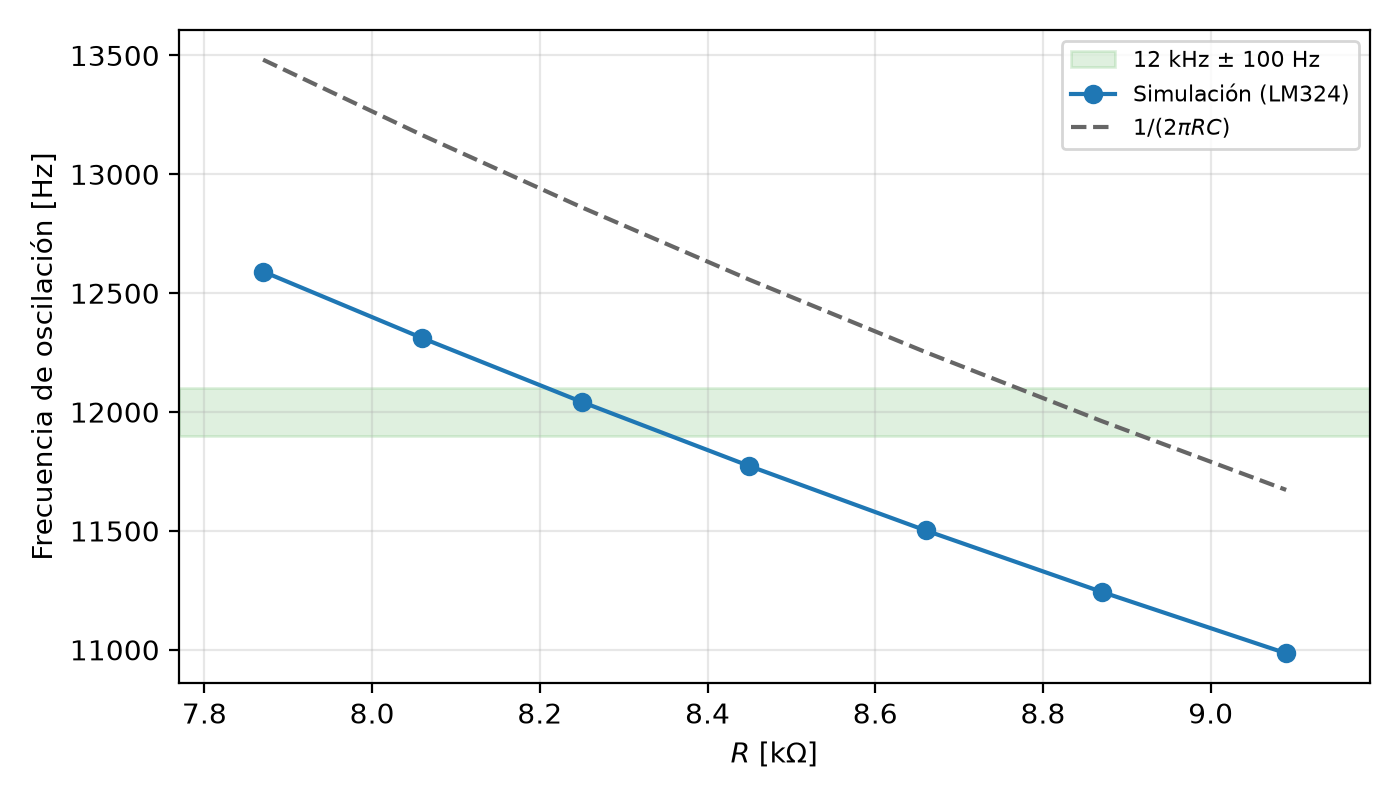
\includegraphics[width=0.7\textwidth]{osc_ajuste_R.png}
    \caption{Frecuencia de oscilación en función de $R$, simulada y teórica.}
    \label{fig:osc_ajuste}
\end{figure}

Con el valor teórico ($8.87 \, [k\Omega]$ en la serie E96) el circuito oscila en $11244 \, [Hz]$, un $6 \, [\%]$ por debajo de lo esperado, como anticipaba el análisis de fase. Se adopta $R = 8.25 \, [k\Omega]$, con el que la frecuencia resulta $12042.6 \, [Hz]$, dentro de la tolerancia de $\pm 100 \, [Hz]$.

\subsection{Simulación}
\label{sec_5.4}
El circuito se simuló con el macromodelo \texttt{LM324/NS} y diodos 1N4148, partiendo de una condición inicial de $10 \, [mV]$ en la entrada no inversora. La oscilación crece y se estabiliza en menos de $1 \, [ms]$ (\autoref{fig:osc_arranque}).

\begin{figure}[H]
    \centering
    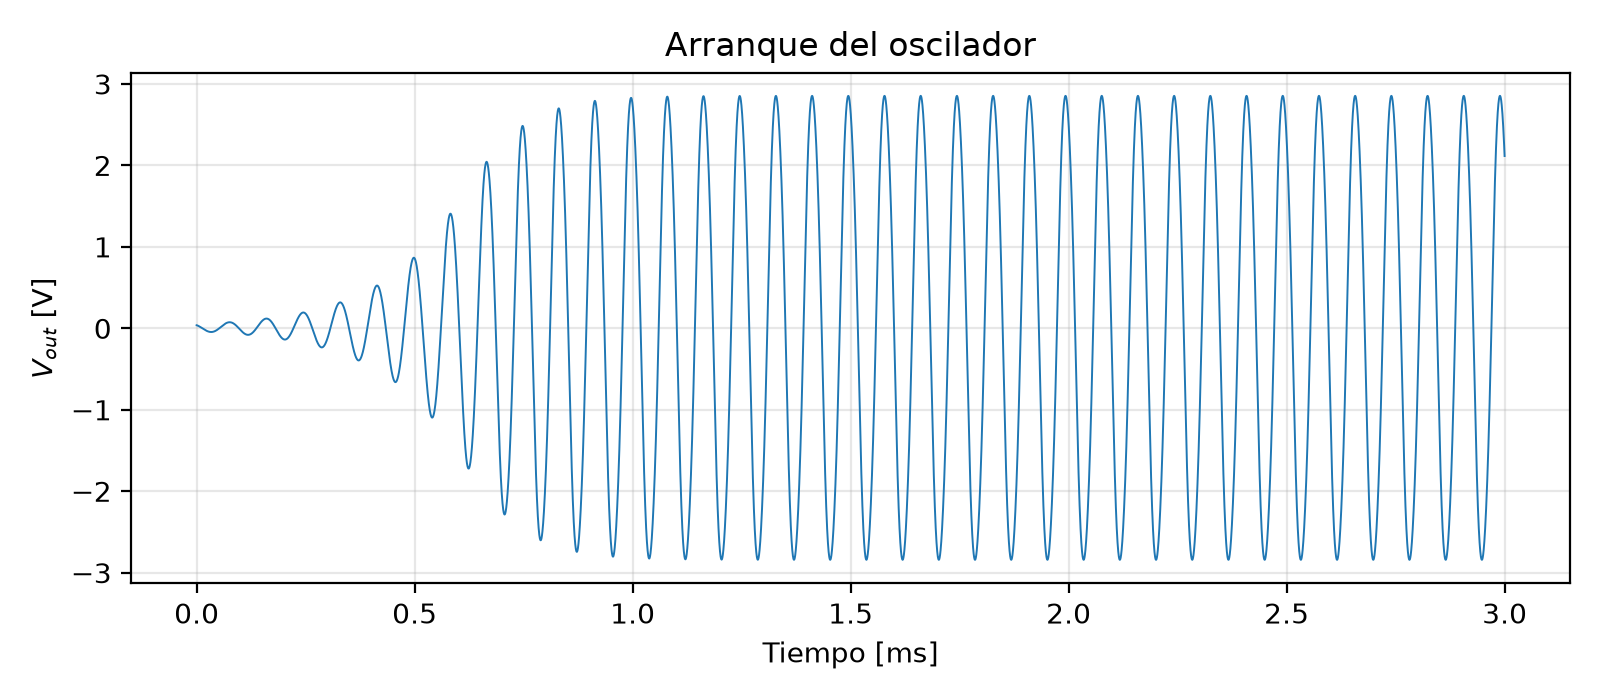
\includegraphics[width=0.8\textwidth]{osc_arranque.png}
    \caption{Arranque del oscilador.}
    \label{fig:osc_arranque}
\end{figure}

\begin{figure}[H]
    \centering
    \begin{subfigure}{0.49\textwidth}
        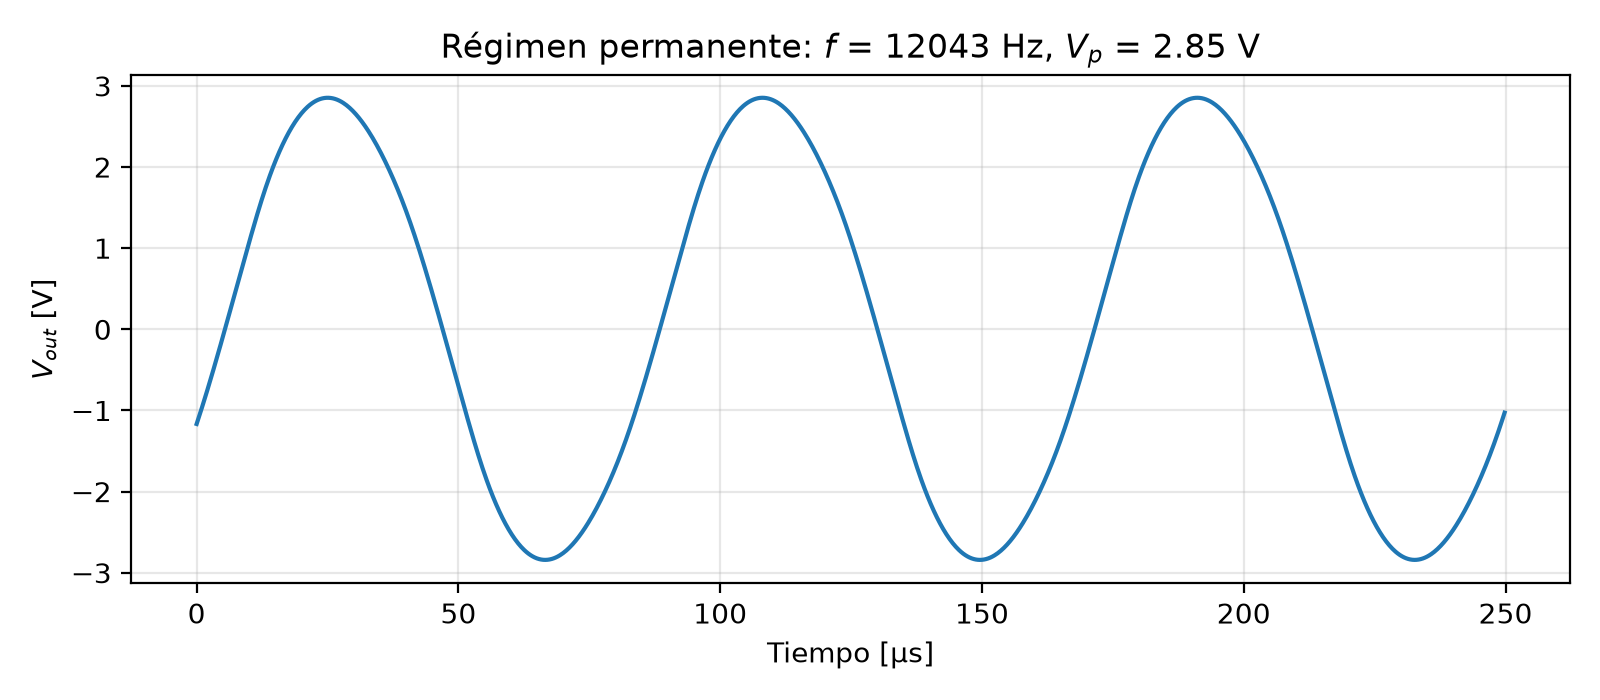
\includegraphics[width=\textwidth]{osc_permanente.png}
        \caption{Régimen permanente.}
        \label{fig:osc_perm}
    \end{subfigure}
    \hfill
    \begin{subfigure}{0.49\textwidth}
        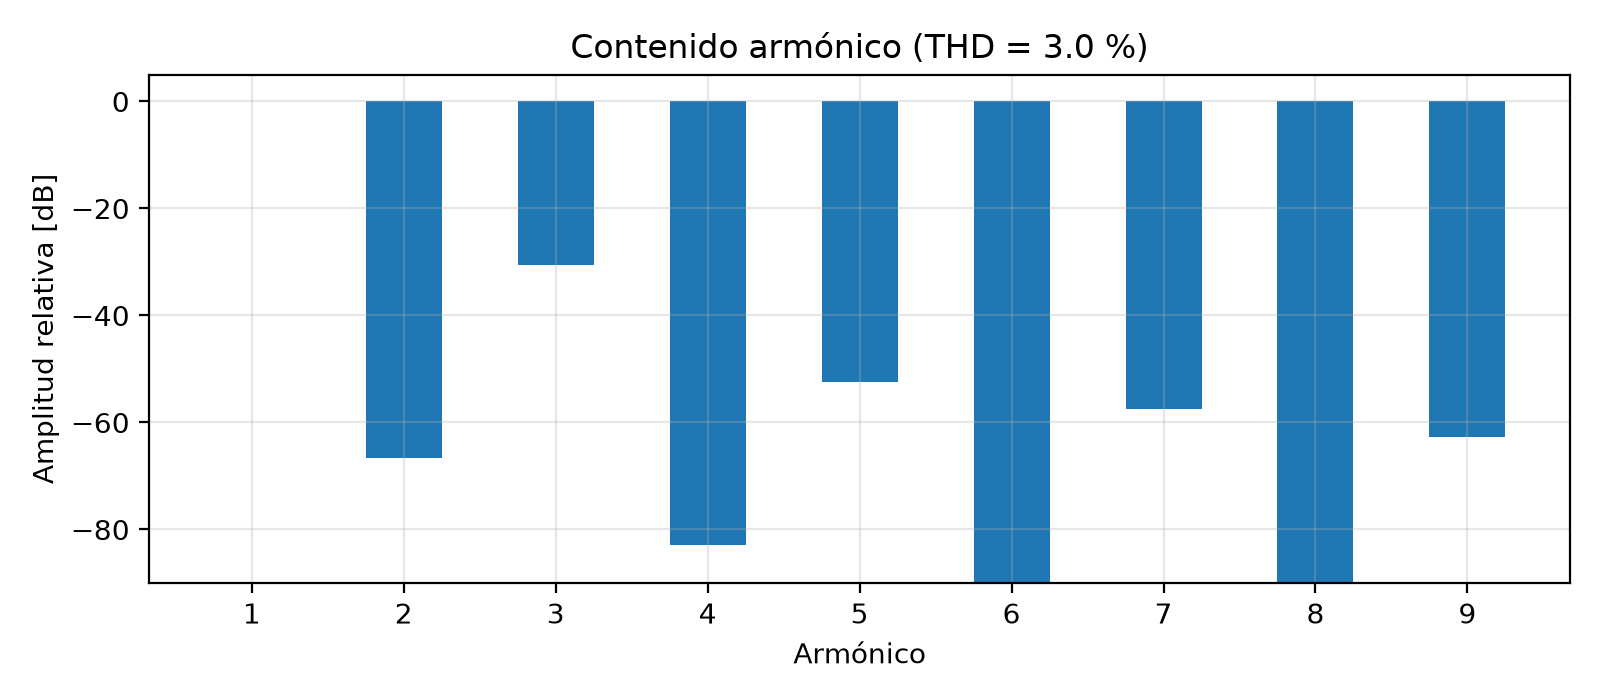
\includegraphics[width=\textwidth]{osc_espectro.png}
        \caption{Contenido armónico.}
        \label{fig:osc_espectro}
    \end{subfigure}
    \caption{Tensión de salida en régimen permanente.}
\end{figure}

En régimen permanente la amplitud es de $2.85 \, [V]$ de pico, en acuerdo con la estimación de la \autoref{eq:amplitud}. La distorsión armónica total, calculada sobre $9$ armónicos mediante un ajuste por mínimos cuadrados sobre los últimos $10 \, [ms]$, es del $3.0 \, [\%]$, dominada por el tercer armónico ($-30.5 \, [dB]$), como corresponde a la alinealidad simétrica de los diodos.

\begin{table}[H]
    \centering
    \caption{Resultados del oscilador.}
    \label{tab:osc}
    \begin{tabular}{|l|c|}
        \hline
        \textbf{Parámetro} & \textbf{Valor} \\
        \hline
        Frecuencia de oscilación & $12042.6 \, [Hz]$ ($+0.35 \, [\%]$) \\
        Amplitud de salida & $2.85 \, [V]$ de pico \\
        Distorsión armónica total & $3.0 \, [\%]$ \\
        Tiempo de establecimiento & $< 1 \, [ms]$ \\
        \hline
    \end{tabular}
\end{table}

\subsection{Verificación del Límite por Slew Rate}
\label{sec_5.5}
Para mostrar por qué la amplitud debe limitarse, se simuló el circuito con $R_{f1} = 18 \, [k\Omega]$ y $R_{f2} = 4.7 \, [k\Omega]$, que llevan $R_{f2,ef}$ a $2 \, [k\Omega]$ y la amplitud prevista por la \autoref{eq:amplitud} a unos $7.5 \, [V]$. La simulación da $7.54 \, [V]$ de pico. La \autoref{fig:osc_slew} compara ambas versiones junto con la derivada de la salida: con la red elegida la pendiente máxima es de $0.23 \, [V/\mu s]$, mientras que con la red alternativa la derivada se aplana en $\pm 0.49 \, [V/\mu s]$ cerca de los cruces por cero, es decir, el amplificador trabaja a su velocidad máxima.

\begin{figure}[H]
    \centering
    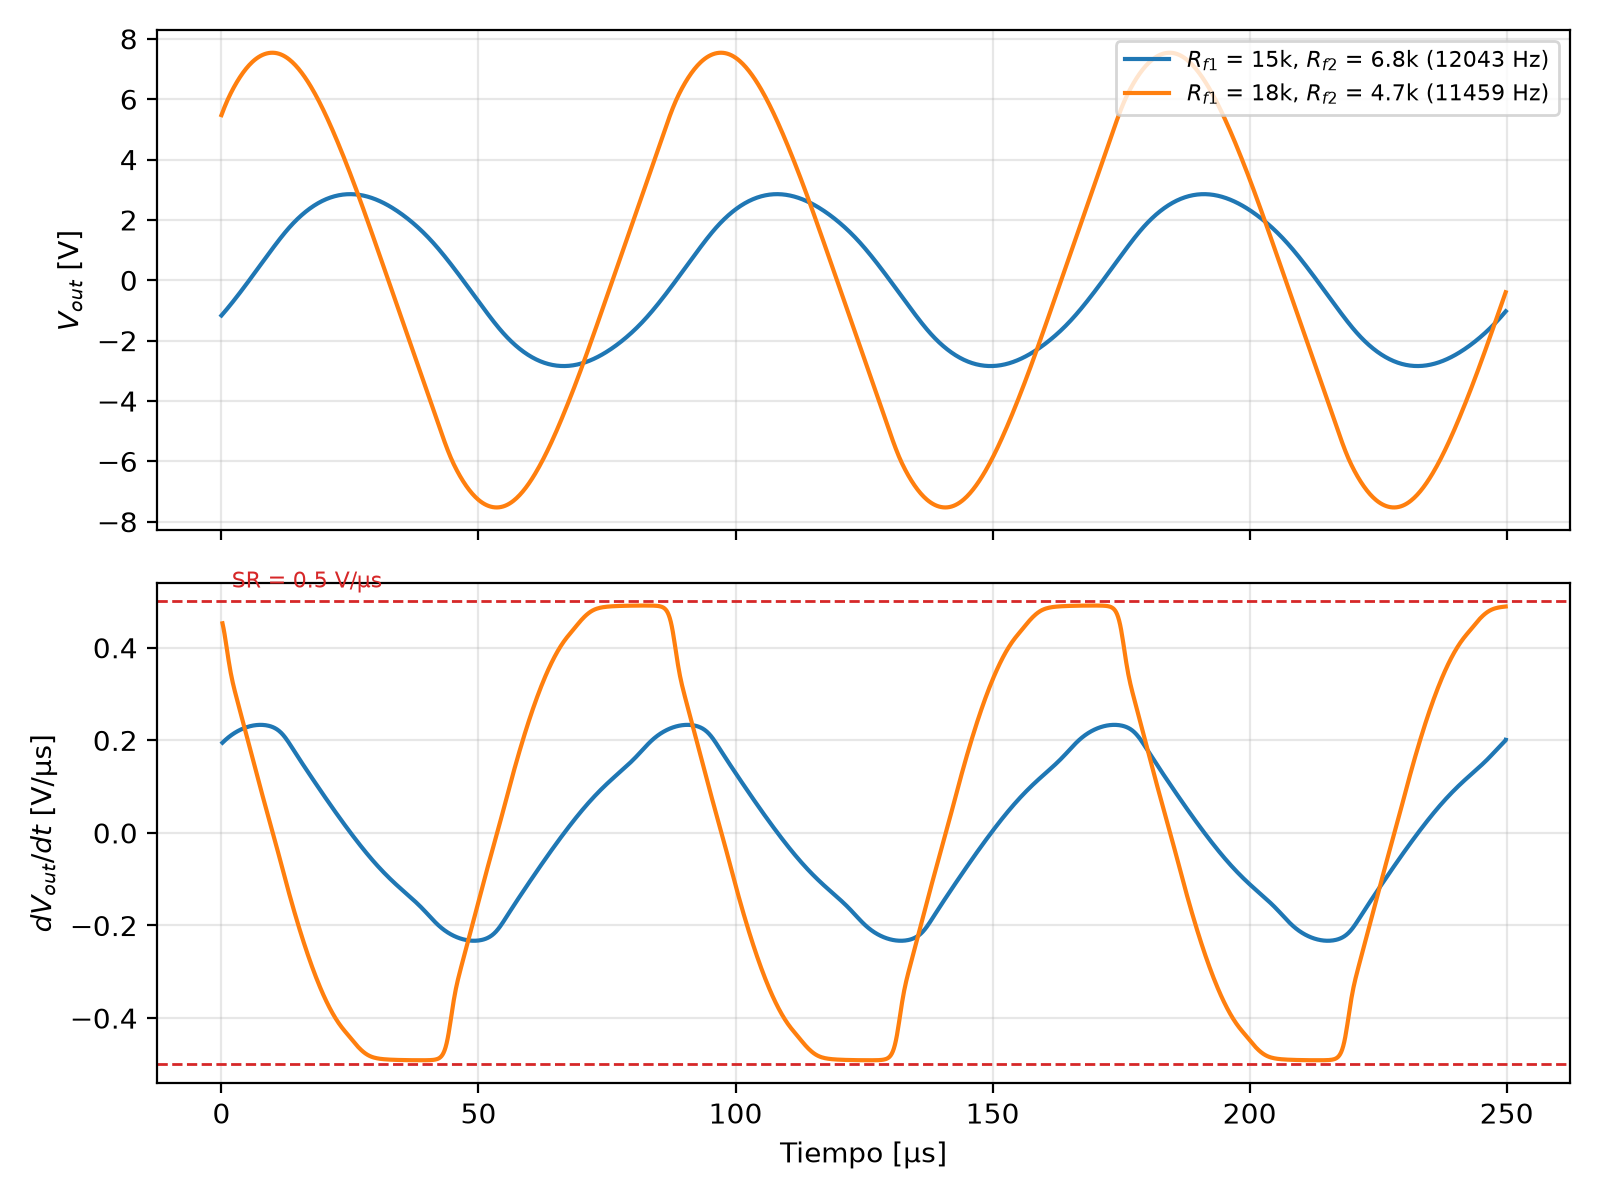
\includegraphics[width=0.8\textwidth]{osc_slew_rate.png}
    \caption{Salida y derivada de la salida para las dos redes de control de amplitud.}
    \label{fig:osc_slew}
\end{figure}

Como la senoidal de $7.54 \, [V]$ requeriría $2\pi \cdot 11.46 \, [kHz] \cdot 7.54 \, [V] = 0.54 \, [V/\mu s]$, apenas un $8 \, [\%]$ más que el \textit{slew rate}, la forma de onda se deforma poco a simple vista. El efecto principal es sobre la frecuencia: el retardo adicional la hace caer a $11459 \, [Hz]$, $584 \, [Hz]$ por debajo del diseño y fuera de la tolerancia pedida.

\subsection{Sensibilidad a las Tolerancias}
\label{sec_5.6}
Como $f_0 \propto (R_1 R_2 C_1 C_2)^{-1/2}$, la sensibilidad de la frecuencia respecto de cada elemento de la red es $-1/2$. Para estimar su efecto se realizó un Montecarlo de $100$ corridas con resistores del $1 \, [\%]$ y capacitores del $5 \, [\%]$ (\autoref{fig:osc_mc}). La frecuencia resultó de $12031 \pm 239 \, [Hz]$ (entre $11546$ y $12645 \, [Hz]$), y solo el $30 \, [\%]$ de los circuitos quedó dentro de $\pm 100 \, [Hz]$.

\begin{figure}[H]
    \centering
    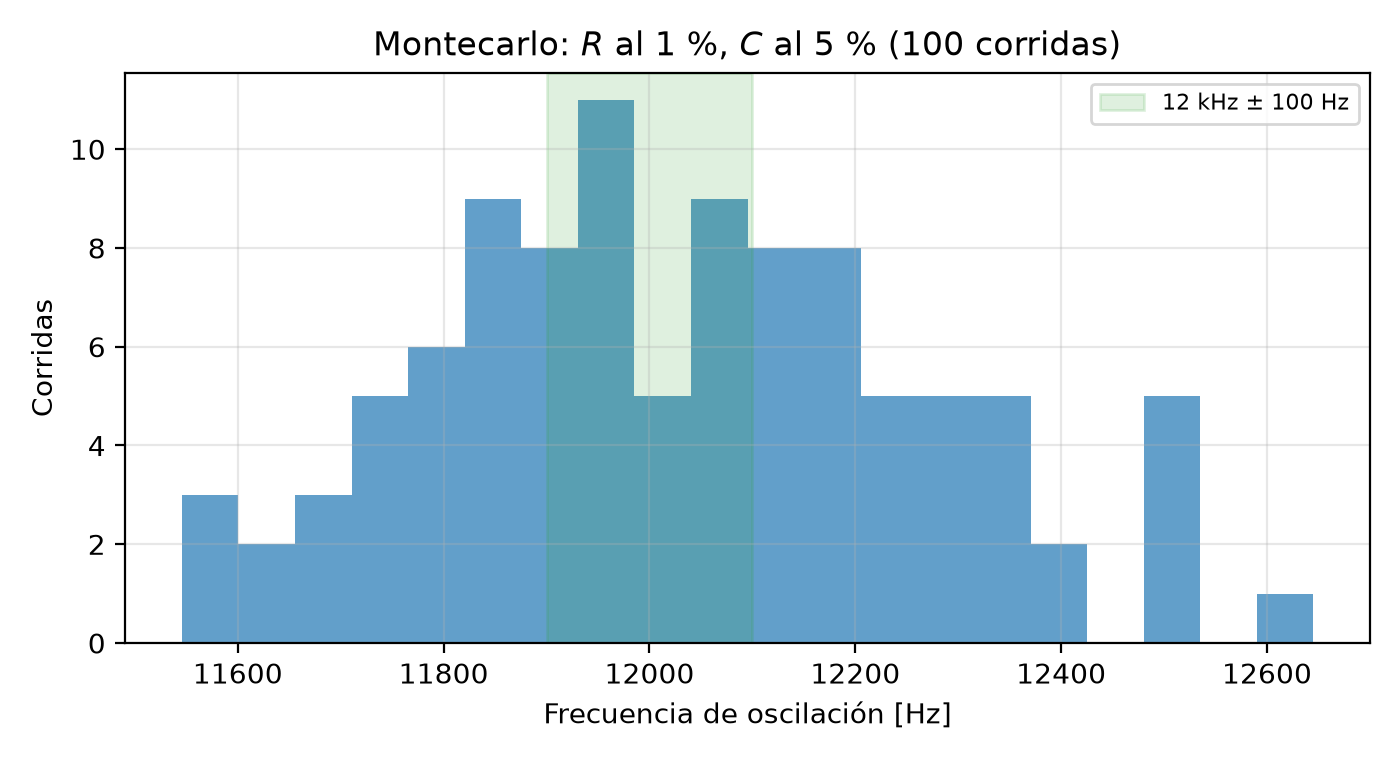
\includegraphics[width=0.7\textwidth]{osc_montecarlo.png}
    \caption{Distribución de la frecuencia de oscilación con $R$ al $1 \, [\%]$ y $C$ al $5 \, [\%]$.}
    \label{fig:osc_mc}
\end{figure}

Por lo tanto, en una implementación física es necesario un elemento de ajuste, por ejemplo reemplazar $R_2$ por una resistencia de $7.5 \, [k\Omega]$ en serie con un preset de $1 \, [k\Omega]$. La variación de $R_2$ altera levemente la atenuación de la red, pero el lazo de control de amplitud lo compensa.

\newpage

\section{Conclusiones}
\label{sec_6}
Se sintetizó un filtro pasabanda a partir de la plantilla de la Cátedra. La aproximación de Chebyshev de orden $2$, transformada a un pasabanda de orden $4$, coincide con la función de transferencia de referencia y ofrece $34.8 \, [dB]$ de atenuación en ambas bandas de rechazo. Se implementó con dos celdas Sallen-Key de componentes iguales ($k = 2.609$), un pasabajos en $1296 \, [Hz]$ y un pasaaltos en $771.5 \, [Hz]$, más un divisor con seguidor para ajustar la ganancia, utilizando tres de los cuatro amplificadores de un LM324. La simulación nominal reproduce la respuesta teórica: cumple el rechazo con más de $4.5 \, [dB]$ de margen, y el rizado resulta de $0.273 \, [dB]$ frente a los $0.25 \, [dB]$ especificados, diferencia que se debe a la cuantización de los valores normalizados.

El análisis de sensibilidad muestra la debilidad del diseño de componentes iguales. Aunque las sensibilidades de $\omega_p$ son de $-1/2$, las del ancho de banda llegan a $5.1$ respecto de los componentes y a $6.7$ respecto de $k$, porque el coeficiente de $s$ es proporcional a la diferencia $3 - k = 0.39$. Con componentes del $10 \, [\%]$ la frecuencia de los polos puede desplazarse entre $-17 \, [\%]$ y $+24 \, [\%]$, y el peor caso del ancho de banda es todavía más grave: en un sentido el $Q_p$ cae a $0.87$ y el rechazo no se cumple; en el otro, $k$ llega a $2.97$ y los polos pasan al semiplano derecho, de modo que el filtro oscila. La simulación de Montecarlo confirmó que esto no es un caso extremo improbable: el $8 \, [\%]$ de los circuitos con componentes del $10 \, [\%]$ resultó inestable.

El estudio de tolerancias mostró que el rechazo de $30 \, [dB]$ se cumple con holgura desde el $5 \, [\%]$, mientras que el rizado de $0.25 \, [dB]$ prácticamente no se alcanza ni con componentes del $1 \, [\%]$. Esta conclusión es propia de la aproximación de Chebyshev: al ser la solución óptima para el orden dado, su rizado nominal coincide con el límite y cualquier desvío lo excede. Para un armado real convendría diseñar con un rizado menor que el especificado, aprovechando el margen en las bandas de rechazo, o prever un ajuste de cada etapa.

La comparación con la topología de ganancia unitaria, con la misma función de transferencia, muestra que esta es claramente más robusta: la suma de las sensibilidades del ancho de banda baja de $13.3$ a $2$, no puede volverse inestable y, con componentes del $10 \, [\%]$, la mediana del rizado baja de $4.0$ a $0.9 \, [dB]$. Su costo es una mayor dispersión de valores ($C_1/C_2 = 26$). El amplificador real, por su parte, agrega unos $0.05 \, [dB]$ de rizado y limita la atenuación por encima de $40 \, [kHz]$, sin comprometer la especificación.

La automatización de las simulaciones con Python y \texttt{spicelib} fue la herramienta que hizo posibles estos análisis. A partir de los esquemáticos dibujados en LTspice, un único script ejecuta todas las simulaciones del trabajo (más de $3000$ corridas) en unos tres minutos, con resultados idénticos a los de las simulaciones manuales. Generar los valores desde Python permitió además calcular los polos de cada corrida y detectar la inestabilidad, que el análisis AC por sí solo no revela, y guardar los resultados permitió regenerar e inspeccionar las figuras sin volver a simular.

Por último, se diseñó un oscilador puente de Wien que, con $R = 8.25 \, [k\Omega]$ y $C = 1.5 \, [nF]$, oscila en $12042.6 \, [Hz]$, dentro de la tolerancia de $\pm 100 \, [Hz]$, con $2.85 \, [V]$ de amplitud y $3 \, [\%]$ de distorsión. El ajuste en simulación fue imprescindible, porque el retardo de fase del LM324 baja la frecuencia un $6 \, [\%]$ respecto de $1/(2\pi RC)$. También se verificó que la amplitud debe mantenerse por debajo del límite que impone el \textit{slew rate}, y que con componentes comerciales hace falta un preset para alcanzar la tolerancia pedida.


\newpage
\nocite{*}
\printbibliography[heading=bibintoc, title={Bibliografía y Referencias}]
\end{document}
